
\hspace{0pt}
\vfill

\invisiblesection{Cover page}

\begin{center}
    {\huge First Partial Project:\\Graph Search Algorithms}\\    \quad\\
    {\large Universidad Panamericana}\\
    {\large Facultad de Ingeniería}\\
    \quad\\
    \quad\\
    
\includegraphics[scale=0.3]{../img/UP}
    \quad\\
    \quad\\
    Inteligencia Artificial\\
    Dr. Ari Yair Barrera Animas\\
    \quad\\
    \quad\\
    \begin{tabular}{c|c}
        Osornio López Daniel Alejandro & 0244685\\
		Daniel Hernandez Toledo & 
    \end{tabular}\\
    \quad\\
    \quad\\
	02-22-2022
\end{center}

\vfill

\newpage
\invisiblesection{Contents}
\tableofcontents

\newpage
\section{Objectives}

1. Design and implement search algorithms for graph structures using
the Rust programming language

\begin{enumerate}[label={}]
\item 1.1 Breadth First
\item 1.2 Uniform Cost (Dijkstra)
\item 1.3 Depth First
\item 1.4 Limited Depth First
\item 1.5 Iterative Depth First
\item 1.6 Bidirectional
\end{enumerate}



2. Correct and efficient documentation of the code and features


\section{Abstract}


\newpage
\section{Installation \& Execution}

The programming language we chose is Rust, it is a compiled,
general purpose, low-level systems language with a strong type system,
no garbage collector nor manual allocators but a lifetime borrow-checker that
makes code compiled with it memory safety, performant as C but with high-level
abstractions like with zero-cost abstractions.

\subsection{Install Rust}

To install rust, on Unix-like systems only the following command is needed:

\begin{minted}{bash}
curl --proto '=https' --tlsv1.2 -sSf https://sh.rustup.rs | sh
\end{minted}

After the installation is finished, we must add \texttt{\$HOME/.cargo/bin} to the \texttt{\$PATH}.
Yo may want to restart your terminal emulator for the changes to the \texttt{\$PATH} to take effect.

More information at \texttt{https://www.rust-lang.org/tools/install}

\subsection{Install the program}

\subsubsection{Install from crates.io}

\texttt{crates.io} is the Rust community’s crate registry which allows users to publish and download \textit{crates}.
A crate is a compilation unit in Rust, like a library or an executable binary.

To install the program from \texttt{crates.io} use \texttt{cargo}, the Rust package manager.

\begin{minted}{bash}
cargo install aigraph1
\end{minted}

The command \texttt{aigraph1} should be available from the command prompt.
To execute the program run the command \texttt{aigraph1} in the terminal prompt.

\subsubsection{Install from GitHub}

The source code within the GitHub repository is the same the team sent you via the Moodle assignment.
We can either use \texttt{cargo} to compile from GitHub automatically or manually clone the repository and
compile.

To install using the source code from GitHub with a single command use:
\begin{minted}{bash}
cargo install --git https://github.com/AOx0/aigraph1
\end{minted}

Otherwise, to compile/install manually. First, clone the GitHub repository and move inside the created directory.

\begin{minted}{bash}
git clone https://github.com/AOx0/aigraph1 && cd ./airgraph1
\end{minted}

Now we can either install the program to \texttt{\$HOME/cargo/.bin} or run it in-place. When compiling a 
Rust program every temporary file and binary is placed inside a \texttt{target} directory. To clean everything
related to the project, just remove the target directory inside aigraph1.

Execute the following command to install the binary;

\begin{minted}{bash}
cargo install --path .
\end{minted}

The command \texttt{aigraph1} should be available from the command prompt.
To execute the program run the command \texttt{aigraph1} in the terminal prompt.

The alternative is to run in-place. For this purpose use the following command inside the \texttt{aigraph1} directory:

\begin{minted}{bash}
cargo run --release
\end{minted}

This command will compile and run the project.

\subsubsection{Install from source code}

The source code in the zip file is the same as in GitHub. To run or install the program unzip the file and move inside the
directory.


\begin{minted}{bash}
unzip -q aigrap1.zip && cd ./aigraph1
\end{minted}


Now we can either install the program to \texttt{\$HOME/cargo/.bin} or run it in-place. When compiling a 
Rust program every temporary file and binary is placed inside a \texttt{target} directory. To clean everything
related to the project, just remove the target directory inside aigraph1.

Execute the following command to install the binary;

\begin{minted}{bash}
cargo install --path .
\end{minted}

The command \texttt{aigraph1} should be available from the command prompt.
To execute the program run the command \texttt{aigraph1} in the terminal prompt.

The alternative is to run in-place. For this purpose use the following command inside the \texttt{aigraph1} directory:

\begin{minted}{bash}
cargo run --release
\end{minted}

This command will compile and run the project.


\newpage
\section{Dependencies}

There are two types of dependencies in the project, for benchmarking and graph related.

\subsection{Graph dependencies}

\subsubsection{petgraph v0.6.3}

Graphs are collections of nodes, and edges between nodes. \texttt{petgraph} provides several graph types 
(each differing in the tradeoffs taken in their internal representation), algorithms on those graphs, 
and functionality to output graphs in \texttt{graphviz} format. Both nodes and edges can have arbitrary associated data, 
and edges may be either directed or undirected. \autocite{petgraph}

For the graph, the team uses \texttt{petgraph::Graph}, which is a performant adjacency list representation based graph
with an API that identifies nodes and edges with indexes.

\subsubsection{fixedbitset v0.4.2}

\texttt{petgraph} exposes methods that return a \texttt{fixedbitset::FixedBitSet}, which is a collection of bits that can be either 1 (\texttt{true})
or 0 \texttt{false}. \texttt{petgraph} uses these sets, for example, to track nodes that have already been visited.

Some methods of our implementation re-export returned values by \texttt{petgraph}. Thus, it's necessary to know the type, making
\texttt{fixedbitset} a dependency. \autocite{fixedbitset}

\subsection{Benchmark dependencies}

\subsubsection{criterion v0.4.0}

Criterion is a Statistics-driven benchmarking library for Rust that performs millions of iterations to measure code preformance
even for minimal regressions. \autocite{criterion}
 
\subsubsection{iai fork @AlexMikhalev}

Iai is an experimental benchmarking harness that uses Cachegrind to perform extremely precise
single-shot measurements of Rust code.

The fork we used at \texttt{github.com/AlexMikhalev/iai/tree/322cd46} (branch \texttt{'memory\_usage'}) is slighlty
modified to allow setup on bench functions so we measure the exact lines of code we want and not the whole
graph initialization. \autocite{iai}

\newpage
\section{Documentation}

The documentation shown here is a mirror that may be outdated. 
The intent is to show the general idea of the structures and features.

Detailed, up to date documentation at \texttt{https://aox0.github.io/aigraph1/graph/}.

\subsection{graph::Graph}

\begin{minted}[fontsize=\footnotesize]{rust}
pub struct Graph<I, N, E, Ty = Directed, Ix = DefaultIx> {
    pub inner: PGraph<N, E, Ty, Ix>,
    pub nodes: HashMap<I, NodeIndex<Ix>>,
}
\end{minted}

The team implemented a new abstraction layer on top of \texttt{petgraph::Graph} to add high-level identifiers for nodes.
Hence, the end-user instead of handling \texttt{petgraph::NodeIndex} and \texttt{petgraph::EdgeIndex} can just use a string like \texttt{'Arad'}.

The structure is generic over various types including data types binded to Nodes and Edges, node identifier type, graph direction and bit-size of
\texttt{petgraph::NodeIndex} and \texttt{petgraph::EdgeIndex}.

\begin{itemize}
 \item \texttt{I} is the type used for identifying the nodes. Because of its purpose, only values that implement
 \texttt{Copy} are allowed like \texttt{\&'\_ T} or \{\texttt{u8}, \texttt{i8}, \texttt{i16}, \texttt{u16}, ...\}. 
 If the identifier is a number it is better to just use \texttt{petgraph::Graph} since its default
 behaviour is to work identifying nodes with numbers, these numbers are named indexes and don't add any overhead
 like this more high-level API which uses a \texttt{HashMap}.
 \item \texttt{N} is the type used to store values within the graph's nodes
 \item \texttt{E} is the type used to store values within the graph's edges
 \item \texttt{Ty} is the Graph connection type. \texttt{petgraph::Directed} by default
 \item \texttt{Ix} is the number type value used as indexer for Edges and Nodes.
\end{itemize}

\subsection{graph::Graph::breadth\_first}
\begin{minted}[fontsize=\footnotesize]{rust}
pub fn breadth_first(&self, start: I, goal: Option<I>) -> Result<Steps<(), Ix>, ()> { ... }
\end{minted}



\newpage
\section{Conclusiones y Recomendaciones}


\newpage
\section{Bibliografía}
\printbibliography[heading=none]

\newpage
\appendix

\section{Appendix}

Comparación de histograma de las ocurrencias de bytes entre un arreglo de bytes
y su versión cifrada por el \texttt{Método 1}

\begin{figure}[H]
    \centering
    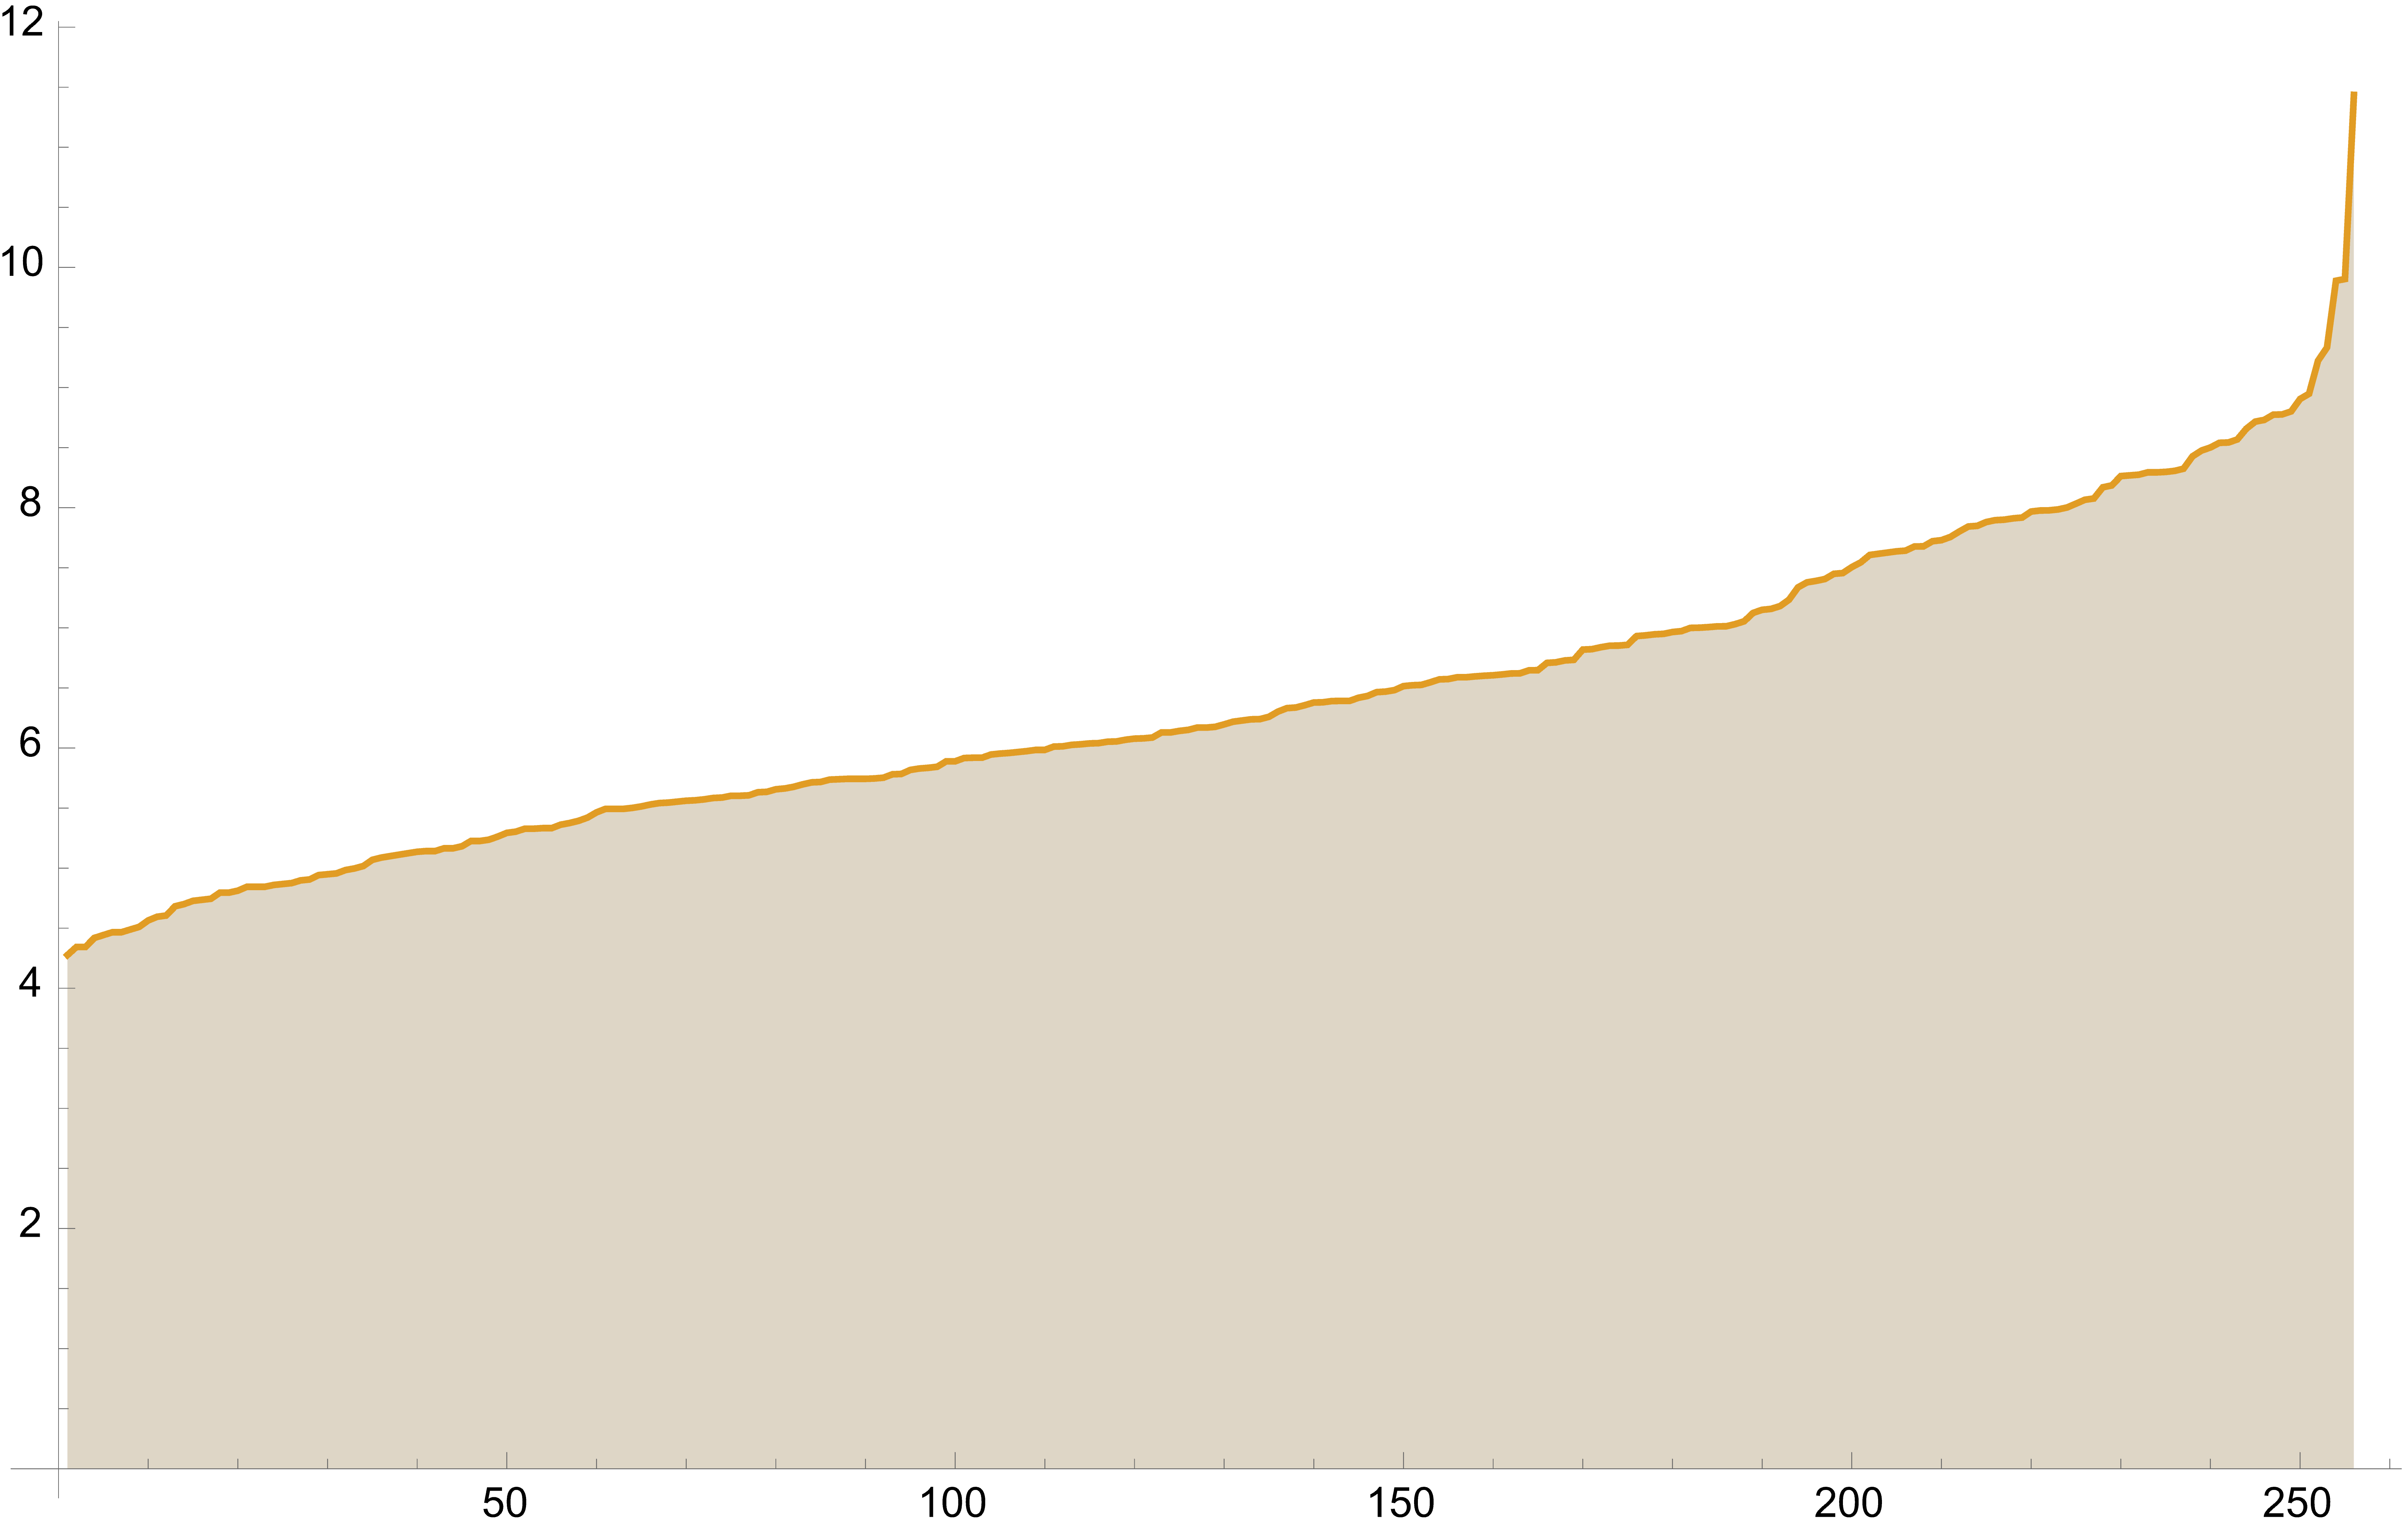
\includegraphics[scale=0.7]{../img/historygram}
    \caption*{Histograma de los bytes del archivo
original y el cifrado.}\label{fig:d2}
\end{figure}

\newpage
\section{Appendix}

